\documentclass[11pt,a4paper,titlepage]{article}
\usepackage[utf8]{inputenc}
\usepackage[english]{babel}
\usepackage[T1]{fontenc}

\usepackage{float}
\usepackage{graphicx}
\usepackage{setspace}
\usepackage{amsmath}
\usepackage{courier}
\usepackage{amsmath}
\usepackage{listings}
\usepackage{color}
\usepackage[toc, page]{appendix}


\definecolor{mygreen}{rgb}{0,0.6,0}
\definecolor{mygray}{rgb}{0.5,0.5,0.5}
\definecolor{mymauve}{rgb}{0.58,0,0.82}




\lstset{ %
	backgroundcolor=\color{white},   % choose the background color
	basicstyle=\footnotesize,        % size of fonts used for the code
	breaklines=true,                 % automatic line breaking only at whitespace
	captionpos=b,                    % sets the caption-position to bottom
	commentstyle=\color{mygreen},    % comment style
	escapeinside={\%*}{*)},          % if you want to add LaTeX within your code
	keywordstyle=\color{blue},       % keyword style
	stringstyle=\color{mymauve},     % string literal style
}

%\renewcommand{\thesubsection}{\thesection.\alph{subsection}}


\usepackage{booktabs}
\usepackage[backend=biber, bibencoding=utf8, style=ieee]{biblatex}

\addbibresource{references.bib}
\usepackage[final,hidelinks]{hyperref} % must be last package loaded

\author{Ólafur Jón Thoroddsen}  % My name, for the titlepage
\title{\includegraphics{graphics/ru-logo}\\\vspace{10mm}
	Mechatronics II\\T-535-MECH \ \\Homework 1}  % The title, for the titlepage

\begin{document}
	\pagenumbering{arabic}
	\maketitle
	
\section{Installing Eclipse for AVR programming on OS~X}

Installation of Eclipse takes a few steps to get right. Using Baldurs embedded C guide\cite{baldurscguide} the process get's a little smoother but for Macs, all the humps have not been resolved.
My computer model and operating system are shown in table~\ref{tab:computer}.

\begin{table}[h]
	\centering
	\begin{tabular}{lr}
		\toprule
		Computer model	&	MacBook Pro (Retina, Mid 2012)\\
		Operating system	&	Mac OS X 10.11.2\\
		\bottomrule
	\end{tabular}
	\caption{System properties}
	\label{tab:computer}
\end{table}


\begin{enumerate}
	\item
	Download the Java Development Kit (JDK) from \url{http://www.oracle.com/technetwork/java/javase/downloads/index.html} and install it into the default directory.
	
	\item
	Download the Arduino software from \url{https://www.arduino.cc/} and copy it to your \verb|/Applications/| directory
	
	\item
	Download Eclipse C/C++ from \url{https://www.eclipse.org/downloads}. I  chose the \textit{Eclipse Installer}, 64 bit version for Mac OS X.
	
	\item
	Install into the default directory
	
	\item
	Download the CrossPack for AVR Development from \url{https://www.obdev.at/products/crosspack/index.html} and install it into the default directory
	
	\item
	Open Eclipse and navigate to $\textbf{Eclipse} \rightarrow \textbf{Preferences} \rightarrow \textbf{AVR} \rightarrow \textbf{Paths}$ and set custom paths as shown in table~\ref{tab:paths}
	
	\begin{table}[h]
		\centering
		\begin{tabular}{ll}
			\toprule
				AVR-GCC		&	/usr/local/CrossPack-AVR/bin\\
				GNU make	&	/usr/bin\\
				AVR Header Files	&	/usr/local/CrossPack-AVR/avr/include\\
				AVRDude	&		/usr/local/CrossPack-AVR/bin\\
			\bottomrule
		\end{tabular}
		\caption{Paths to the AVR compiler, header files, GNU make and AVRDude}
		\label{tab:paths}
	\end{table}

	\item
	\label{item:port}
	Open the Arduino Software, connect your Arduino and navigate to $\textbf{Tools} \rightarrow \textbf{Port}$ and note the Serial port where the Arduino is connected. In my case it connected to \verb|/dev/cu.usbmodem1411|
	
	\item
	In the Eclipse Preferences menu, navigate to $\textbf{AVR} \rightarrow \textbf{AVRDude}$ and tick the box \verb|Use custom configuration for AVRDude| and paste in the following path:
	 \verb|/Applications/Arduino.app/Contents/| \verb|Java/hardware/tools/avr/etc/avrdude.conf|
	If you copied the Arduino software into the \verb|/Applications| directory, this should work, otherwise, replace this with the path to the Arduino.app software.

	\item
	In the AVRDude preferences, add a new Programmer Configuration. Select a name, e.g. "Arduino" and set the options as shown in table~\ref{tab:hardwareconfig}.
	
	\begin{table}[h]
		\centering
		\begin{tabular}{ll}
			\toprule
				Programmer hardware (-c)	&	Arduino\\
				Override default port (-P)	&	The serial port from step~\ref{item:port}\\
				Override default baudrate (-b)	&	115200\\
			\bottomrule
		\end{tabular}
		\caption{Programmer configuration for Arduino}
		\label{tab:hardwareconfig}		
	\end{table}	
	
	\item
	In Eclipse, create a new C project. $\textbf{File} \rightarrow \textbf{New} \rightarrow \textbf{C Project}$. Select a name for the project and choose Project type as \verb|AVR Cross Target| \verb|Application| and the Toolchain as \verb|AVR-GCC Toolchain|.
	
	\item
	Right click on the project folder in the C/C++ Projects pane and choose $\textbf{New} \rightarrow \textbf{Source File}$ and set the name to \verb|main.c|
	
	\item
	Right click on the project folder in the C/C++ Project pane and navigate to $\textbf{Properties} \rightarrow \textbf{AVR} \rightarrow \textbf{Target Hardware}$ and for MCU Type, choose \verb|ATmega328P| (assuming you're using the Arduino Uno R3). Click OK.
	
	\item
	Now you are ready to go!
\end{enumerate}

\section{Blinking an LED}

It's really easy to blink an LED using the Arduino Software. Below are the \verb|setup()| and \verb|loop()| functions from the Blink example provided with the Arduino Software (comments removed for clarity).

\vspace{2mm}
\lstinputlisting[language=C++,frame=single]{Blink/Blink.cpp}
\vspace{2mm}

\noindent Removing the delays will blink the LED on pin 13 as fast as possible. The modified code is shown here below.

\lstinputlisting[language=C++,frame=single]{Blink/Blinkmod.cpp}
\vspace{2mm}

\noindent Using Eclipse it's possible to write more optimized code for the ATmega328P microcontroller on the Arduino. A C program that blinks the LED on pin 13 as fast as possible is shown here below.

\vspace{2mm}
\lstinputlisting[language=C,frame=single,firstline=11]{crazyblink/main.c}
\vspace{2mm} 

\noindent Using an oscilloscope, it's possible to find out how fast the LED is blinking. Results from measurements using both the Arduino code and the C code is shown in table~\ref{tab:results} and figures~\ref{fig:arduino} and~\ref{fig:eclipse}. Notice how the last three periods of the Arduino waveform is duplicated and overlapped, there is some timing issue there that is hard to know the cause of. Even though the C code signal is not a perfect square  waveform, it is definitely very stable.

\begin{table}[H]
		\centering
		\begin{tabular}{lcc}
			\toprule
			&	Arduino code	& C code\\
			\midrule
			Frequency	&	94,3~kHz	&	3,98~MHz\\
			\bottomrule
		\end{tabular}
		\caption{Blinking an LED using both Arduino code and optimized C code}
		\label{tab:results}
\end{table}

The ratio between the frequencies of the C code and Arduino code is approximately $$\frac{3,98~\text{MHz}}{94,3~\text{kHz}} \approx 42,2 $$
That is, the C code generates pulses, 4220\% faster then the Arduino Code.

\begin{figure}[H]
	\centering
	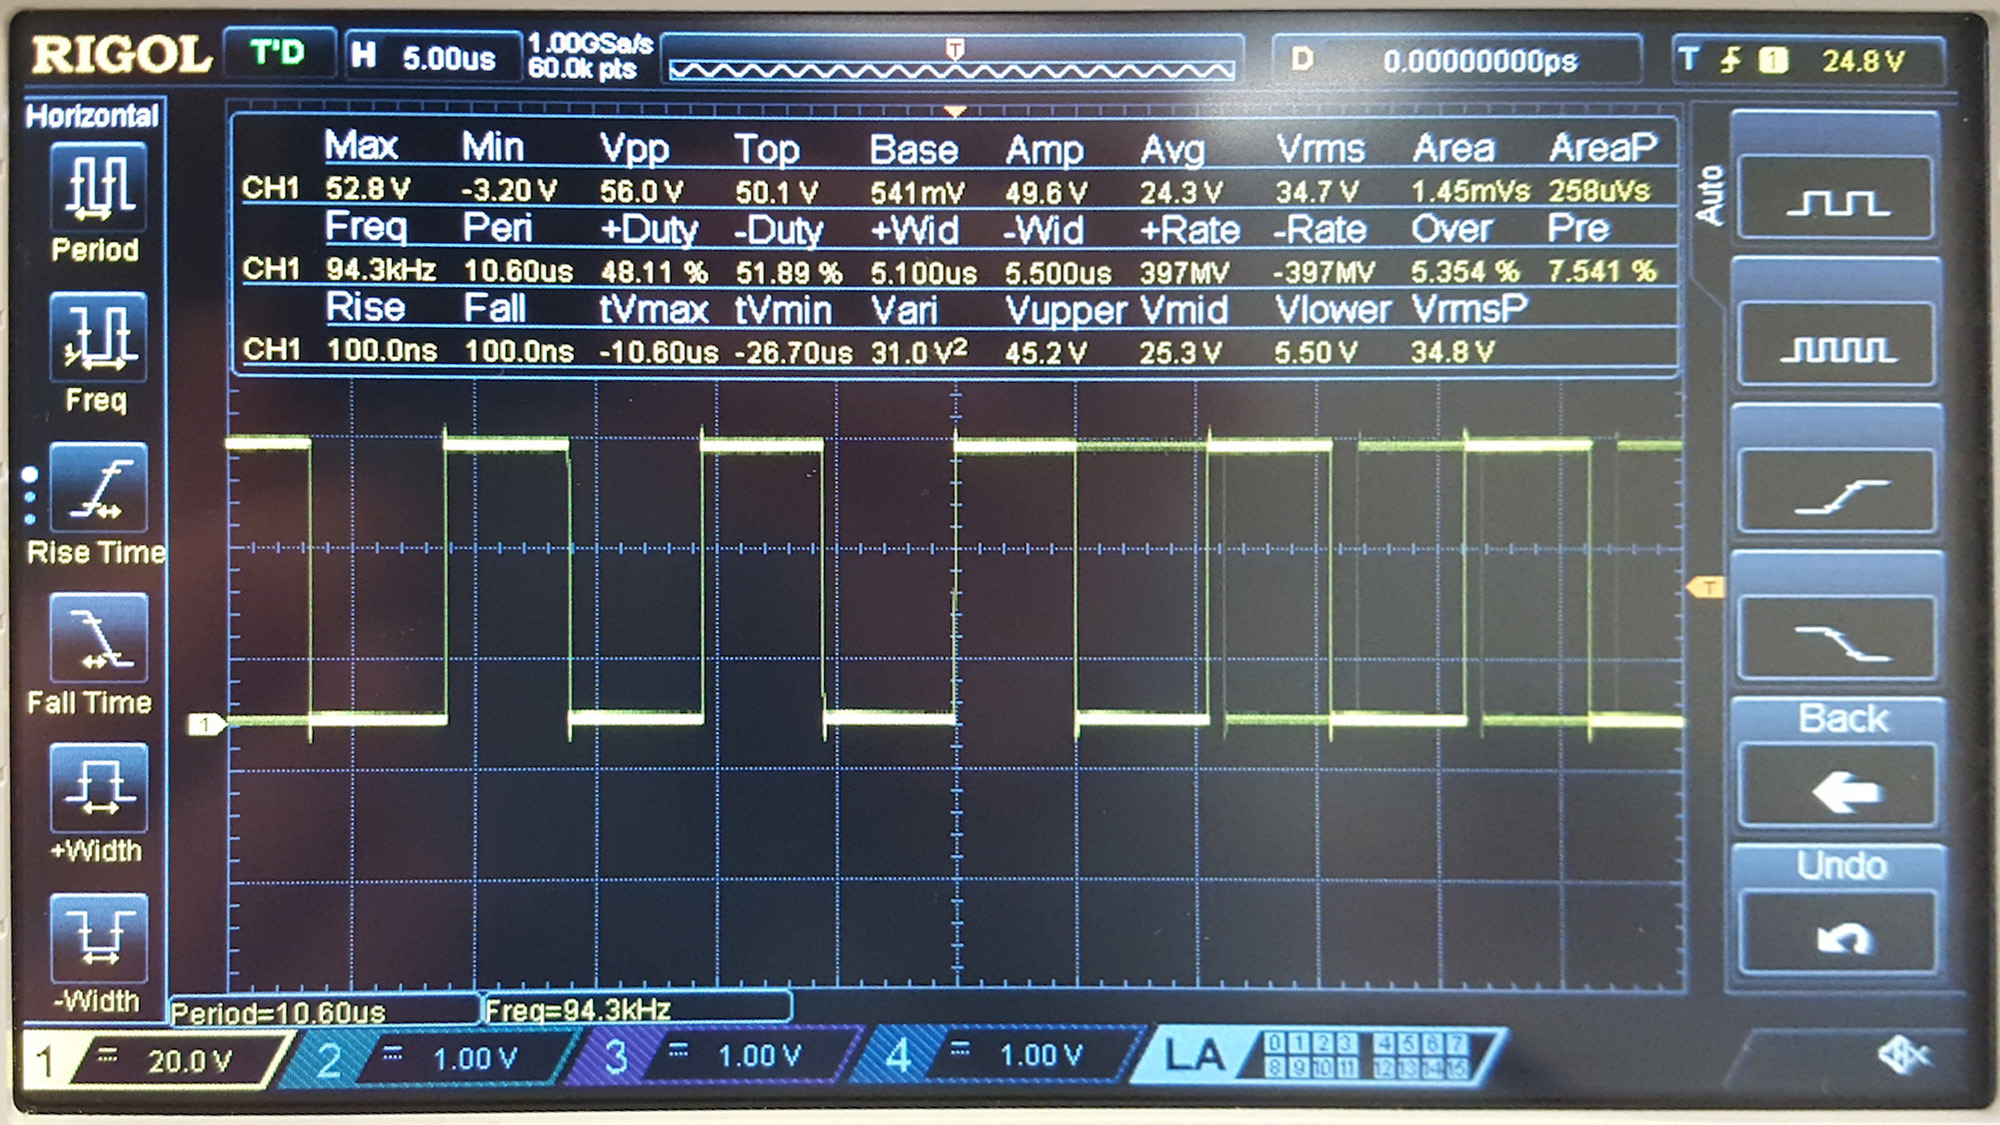
\includegraphics[width=\textwidth]{graphics/arduino_edit}
	\caption{The oscilloscope results from running the Arduino code}
	\label{fig:arduino}
\end{figure}

\begin{figure}[h]
		\centering
		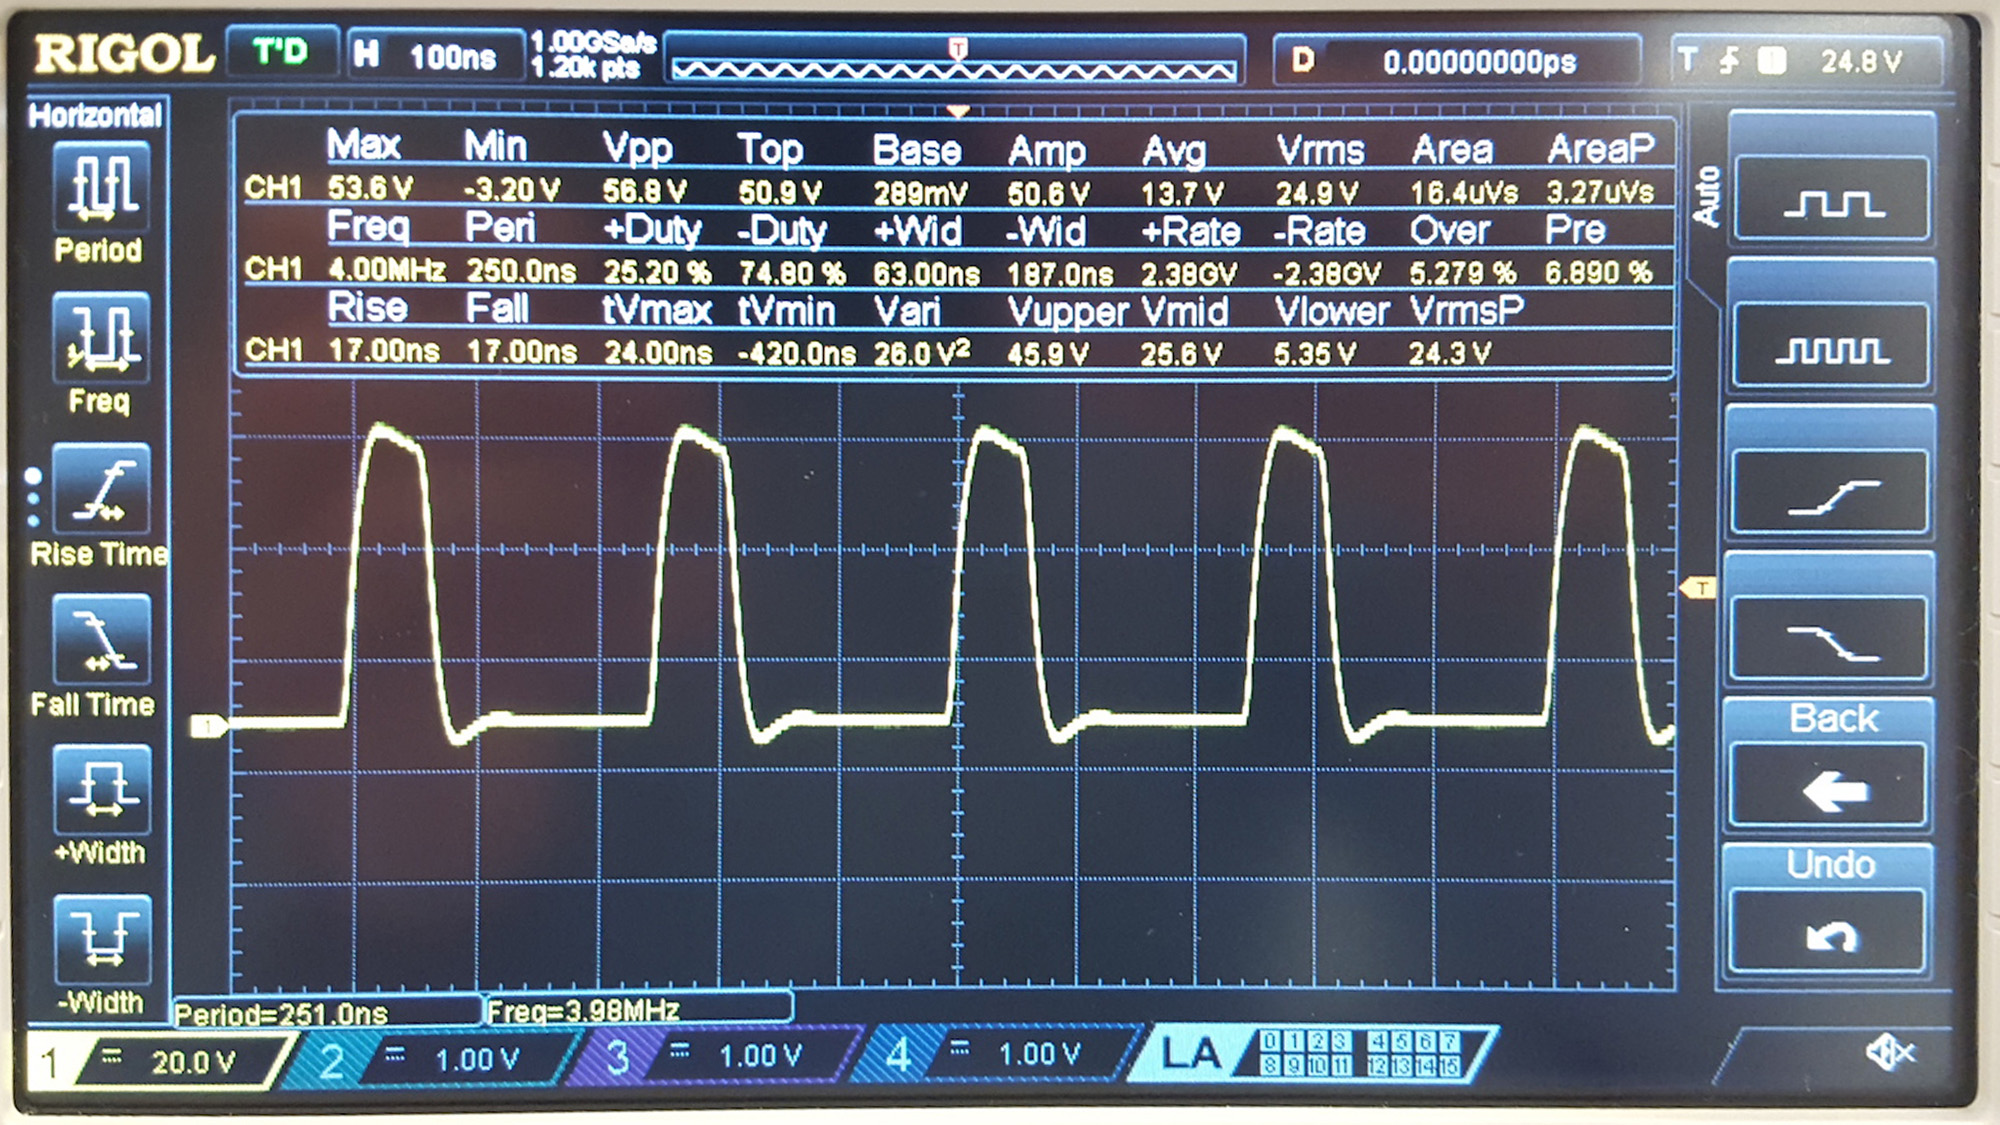
\includegraphics[width=\textwidth]{graphics/eclipse_edit}
		\caption{The oscilloscope results from running the C code}
		\label{fig:eclipse}
\end{figure}

Using raw assembly code, this could maybe be done even faster then demonstrated here. At this time the author does however not posess the knowledge to do so.

\pagebreak

\section{An inverted pendulum}

The working title for my final project will be \textit{An inverted pendulum}. It is about creating my own inverted pendulum robot that can stand on two wheels without falling over. Possible extensions could be to allow it to drive forward and backwards, possibly spin around.

\begin{table}[h]
		\centering
		\begin{tabular}{ll}
			\toprule
			Functional Requirements		&		Design Parameters\\
			\midrule
			React to gravity	&	Motors \& Wheels\\
			Sense it's orientation	&	IMU\\
			Decide how to act	&	PID control software\\
			Power source	&	Batteries\\
			\bottomrule
		\end{tabular}
		\caption{FRs and DPs for an inverted pendulum}
		\label{tab:FRDP}
\end{table}

\begin{table}[H]
		\centering
		\begin{tabular}{cc}
			\toprule
			Risk factor		&	Mitigation\\
			\midrule
			\begin{tabular}{@{}l@{}}I've never used some of\\the components like the\\IMU and PID control software\end{tabular}	&	\begin{tabular}{@{}r@{}}Read up on those \\components in weeks 1~\&~2 \end{tabular}\\
			Time available	&	\begin{tabular}{@{}r@{}}Start early, plan and pivot\\(like they say in entrepreneurship) \end{tabular}\\
			
			\bottomrule
		\end{tabular}
		\caption{Main risk factors and mitigations}
		\label{tab:risks}
\end{table}

\begin{table}[H]
	\centering
	\begin{tabular}{cl}
		\toprule
		Week no.	&	ToDo \& Tests\\
		\midrule
		1	&	Read up on previous work\\
		2	&	\begin{tabular}{@{}l@{}}Research suitable motors and IMUs\\Do an initial design\end{tabular}\\
		3	&	\begin{tabular}{@{}l@{}}Order parts, experiment with\\components I already have\end{tabular}\\
		4	&	\begin{tabular}{@{}l@{}}Start designing the software\\ at a high level (FST)\end{tabular}\\
		5	&	\begin{tabular}{@{}l@{}}Parts should have arrived\\Create experiments for each\\major component. \end{tabular}\\
		\vdots	&	\vdots\\
		\bottomrule
	\end{tabular}
	\caption{Testplan for the inverted pendulum}
	\label{tab:testplan}
\end{table}

This week I will read up on previous work an research suitable motors and IMUs as stated in table~\ref{tab:testplan}.



\pagebreak
\printbibliography

\end{document}